\chapter{基于用户交互的模型改善}
通过自动化算法生成的模型难免含有算法设计者的主观想法在其中,比如树木何时应该分支,何时
应该合并等等。并且算法在处理实际的模型时,通常带有一定的二义性。未免过于主观地决定了模
型的最终成型,本文提倡在自动化生成模型以后,应该将模型
的建立延迟到应用程序,或者使用该模型的最终用户。这样可以使得本文所建立的一系列方法适用于
更广的情形。将自动化算法与人工交互联合使用,可以大大地提高最终模型与具体需求之间的耦合度。

本文根据此需求,开发完成了一个树木模型用户交互平台,可以用于对本文的基于图像所建立的树木
模型进行进一步地编辑和完善。该平台集成了几种不同轻量化级别的模型表示,模型的编辑,算法的
演示等功能,大大的提高了算法验证的直观度和用户与应用级模型改善的方便性。该平台的具体功能
见用例图\ref{fig:usecase}。

\begin{figure}[H]
	\centering
	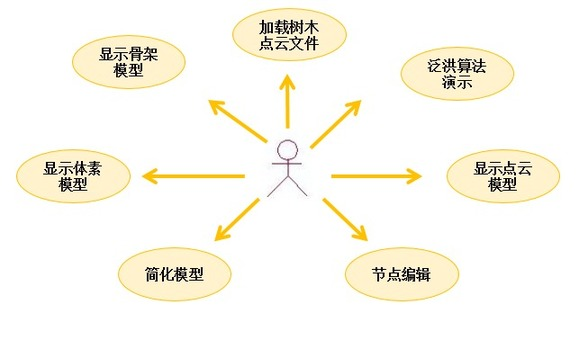
\includegraphics[height=6cm]{usecase.jpg}
	\caption{用户交互平台用例图}
	\label{fig:usecase}
\end{figure}

对于每个用例,本文用表格和图片对其进行进一步说明,由于本文并不将重点放在软件开发上,所以
在本文中未给出具体的系统分析和设计。本文试图对该用户交互平台的功能进行阐述,从而在功能性上
对自动化算法进行人工加强和改善。

\section{交互平台用例说明}
\clearpage
\subsection{加载树木点云文件}

\begin{figure}[H]
	\centering
	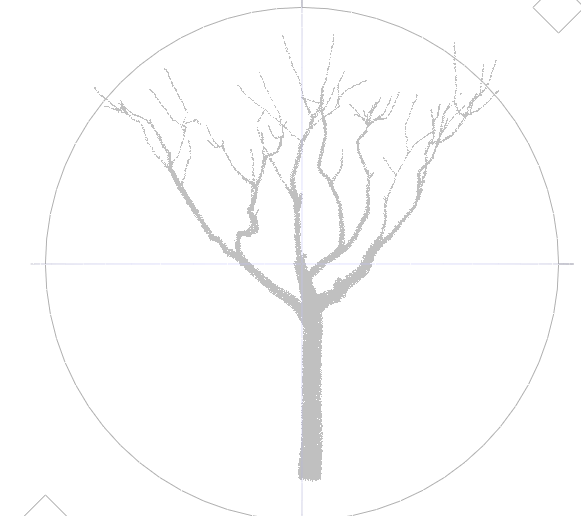
\includegraphics[height=6cm]{uc1.png}
	\caption{用例1图示:用开源软件MeshLab打开的树木点云文件}
	\label{fig:uc1}
\end{figure}

\begin{table}[H]
	\centering
\begin{tabular}{|l|p{8cm}|}
	\hline
	用例名称: & 加载树木点云文件\\
	\hline
	用例标志号: & 1\\
	\hline
	参与者: & 用户\\
	\hline
	简要说明: & 用户可以按键'l'来加载存储为".ply"开源格式的名为"Tree.ply"的点云文件,该
	后缀名的点云模型可以用开源软件Meshlab来打开观察,如图\ref{fig:uc1}\\
	\hline
	前置条件: & 树木的模型文件存在于./Models/文件夹下\\
	\hline
	基本事件流: & 1. 用户按下'l'键\\
	 & 2. 系统去./Models/文件夹下搜索名为"Tree.ply"的点云文件\\
	 & 3. 将点云文件加载入内存\\
	 & 4. 用例终止\\
	\hline
	异常事件流: & 1. 若点云文件不存在,则不会加载入内存\\
	\hline
	后置条件: & 无\\
	\hline
\end{tabular}
\end{table}

\clearpage
\subsection{显示骨架模型}
\begin{figure}[H]
	\centering
	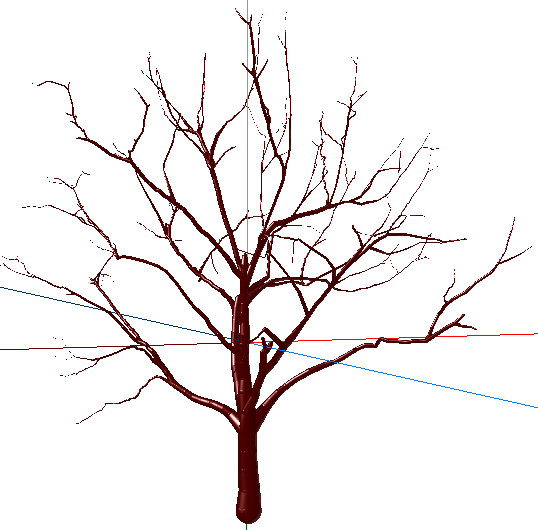
\includegraphics[height=6cm]{uc2.png}
	\caption{用例图示:显示骨架模型}
	\label{fig:uc2}
\end{figure}

\begin{table}[H]
	\centering
\begin{tabular}{|l|p{8cm}|}
	\hline
	用例名称: & 显示骨架模型\\
	\hline
	用例标志号: & 2\\
	\hline
	参与者: & 用户\\
	\hline
	简要说明: & 用户可以通过选择显示骨架模型来观察树木的骨架,具体效果见图\ref{fig:uc2}\\
	\hline
	前置条件: & 树木的模型文件已经被加载进入软件平台\\
	\hline
	基本事件流: & 1. 用户按下'm'键将显示模式切换到骨架模式\\
	 & 2. 将树木骨架模型用冯氏光照模型渲染至视口\\
	 & 3. 用例终止\\
	\hline
	异常事件流: & 1. 若模型文件未加载,则不会显示对应模型骨架\\
	\hline
	后置条件: & 无\\
	\hline
\end{tabular}
\end{table}

\clearpage
\subsection{显示点云模型}
\begin{figure}[H]
	\centering
	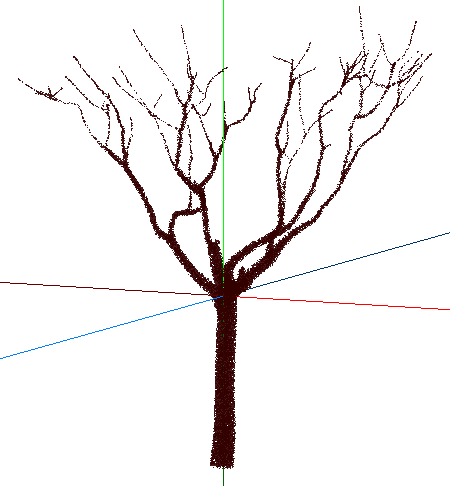
\includegraphics[height=6cm]{uc3.png}
	\caption{用例图示:显示点云模型}
	\label{fig:uc3}
\end{figure}

\begin{table}[H]
	\centering
\begin{tabular}{|l|p{8cm}|}
	\hline
	用例名称: & 显示点云模型\\
	\hline
	用例标志号: & 3\\
	\hline
	参与者: & 用户\\
	\hline
	简要说明: & 用户可以通过选择显示点云模型来观察树木的点云表示,具体效果见图\ref{fig:uc3}\\
	\hline
	前置条件: & 树木的模型文件已经被加载进入软件平台\\
	\hline
	基本事件流: & 1. 用户按下'm'键切换显示模式到点云模式\\
	 & 2. 将点云模型用平滑光照模型渲染至视口\\
	 & 3. 用例终止\\
	\hline
	异常事件流: & 1. 若模型文件未加载,则不会显示对应点云模型\\
	\hline
	后置条件: & 无\\
	\hline
\end{tabular}
\end{table}

\clearpage
\subsection{显示体素模型}
\begin{figure}[H]
	\centering
	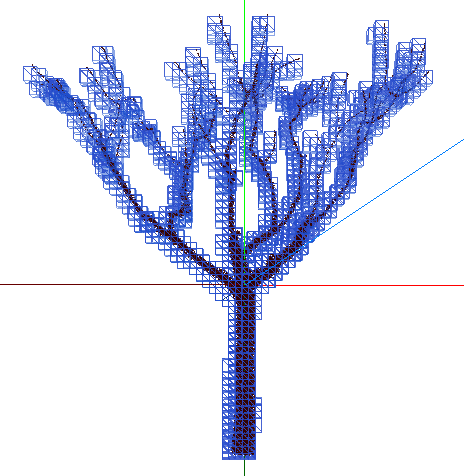
\includegraphics[height=6cm]{uc4.png}
	\caption{用例图示:显示体素模型}
	\label{fig:uc4}
\end{figure}

\begin{table}[H]
	\centering
\begin{tabular}{|l|p{8cm}|}
	\hline
	用例名称: & 显示体素模型\\
	\hline
	用例标志号: & 4\\
	\hline
	参与者: & 用户\\
	\hline
	简要说明: & 用户可以通过选择显示体素模型来观察树木的体素表示,具体效果见图\ref{fig:uc4}\\
	\hline
	前置条件: & 树木的模型已经被加载进入软件平台\\
	\hline
	基本事件流: & 1. 用户按下'v'键\\
	 & 2. 将体素模型用冯氏光照模型渲染至视口\\
	 & 3. 用例终止\\
	\hline
	异常事件流: & 1. 若模型文件不存在,则不会显示对应点云模型\\
	\hline
	后置条件: & 无\\
	\hline
\end{tabular}
\end{table}

\clearpage
\subsection{节点编辑}
\begin{figure}[H]
	\centering
	\subfloat[节点插入(前)]{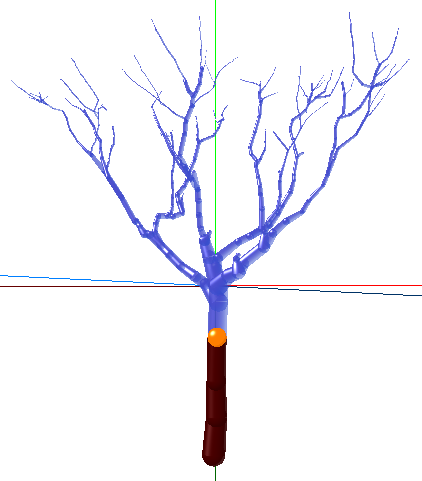
\includegraphics[width=0.26\linewidth]{uc5_ins1.png}}\hfill
	\subfloat[节点删除(前)]{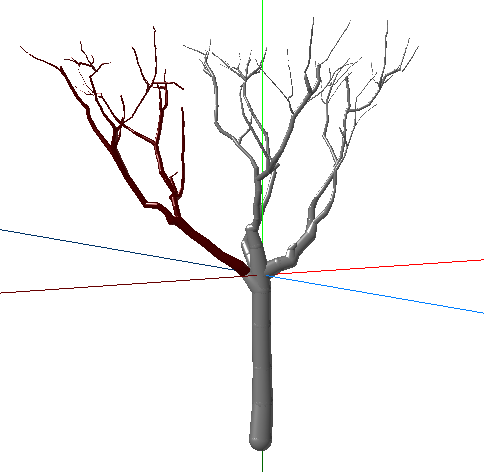
\includegraphics[width=0.26\linewidth]{uc5_rm1.png}}\hfill
	\subfloat[节点移动(前)]{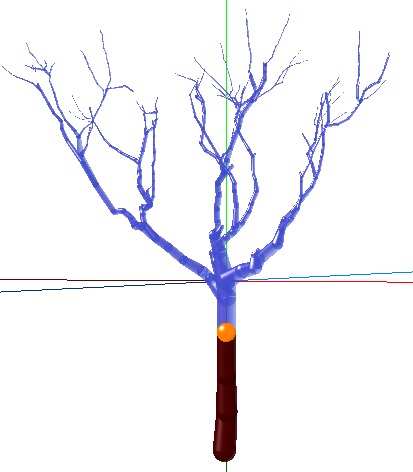
\includegraphics[width=0.26\linewidth]{uc5_mv1.png}}\hfill
	\subfloat[节点插入(后)]{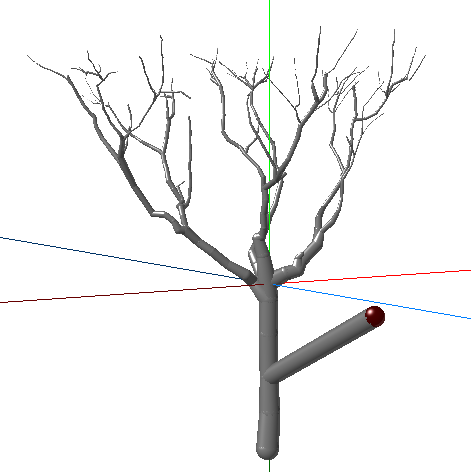
\includegraphics[width=0.26\linewidth]{uc5_ins2.png}}\hfill
	\subfloat[节点删除(后)]{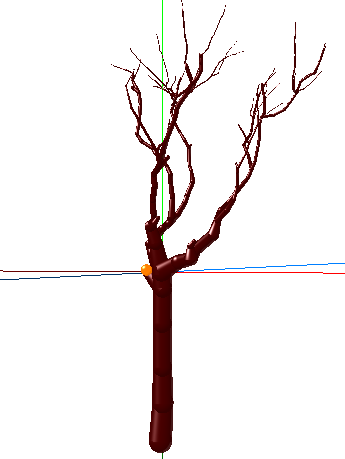
\includegraphics[width=0.26\linewidth]{uc5_rm2.png}}\hfill
	\subfloat[节点移动(后)]{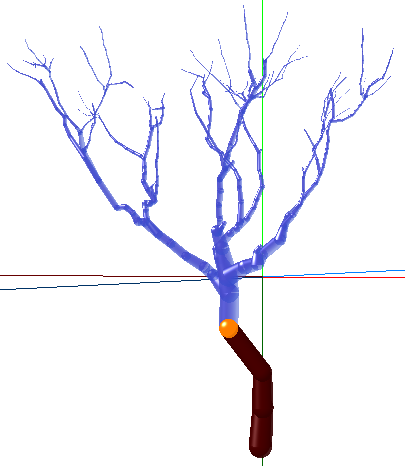
\includegraphics[width=0.26\linewidth]{uc5_mv2.png}}\hfill
	\caption{用例图示:节点编辑}
	\label{fig:uc5}
\end{figure}

\begin{table}[H]
	\centering
\begin{tabular}{|l|p{10cm}|}
	\hline
	用例名称: & 节点编辑\\
	\hline
	用例标志号: & 5\\
	\hline
	参与者: & 用户\\
	\hline
	简要说明: & 可以对选中的节点进行丰富的编辑操作,具体效果见图\ref{fig:uc5}。
	其中橙色球体表示当前选中节点,半透明蓝色部分表示当前节点其下的子树,褐色区域表示树的其他部分\\
	\hline
	前置条件: & 树木的显示模式为骨架模型\\
	\hline
	基本事件流: & 1. 用户按下'g'键\\
	 & 2. 树木骨架从当前节点按用户视角右方向长出一个子节点\\
	 & 3. 调整当前节点为新增的子节点\\
	\hline
	可选事件流1: & 1. 用户按下'p'键\\
	 & 2. 树木删除当前节点以下的子树\\
	\hline
	可选事件流2: & 1. 用户按下鼠标左键拖动\\
	 & 2. 当前节点及其以下的子树在当前平面内平移\\
	\hline
	可选事件流3: & 1. 用户按下'n','f'键\\
	 & 2. 当前节点及其以下的子树在z平面内外平移\\
	\hline
\end{tabular}
\end{table}

\clearpage
\subsection{简化模型}
\begin{figure}[H]
	\centering
	\subfloat[模型简化(前)]{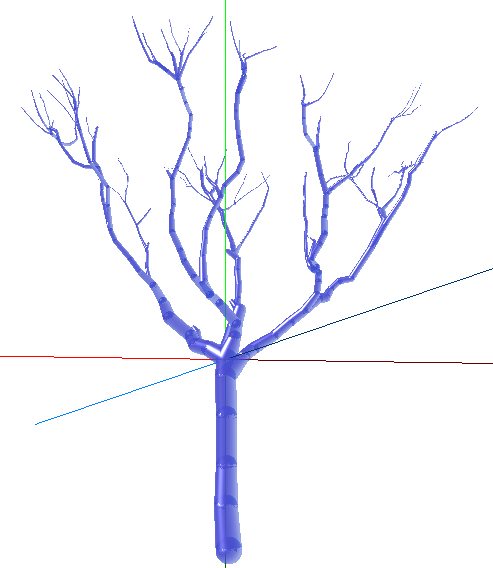
\includegraphics[width=0.4\linewidth]{uc6_1.png}}\hfill
	\subfloat[模型简化(后)]{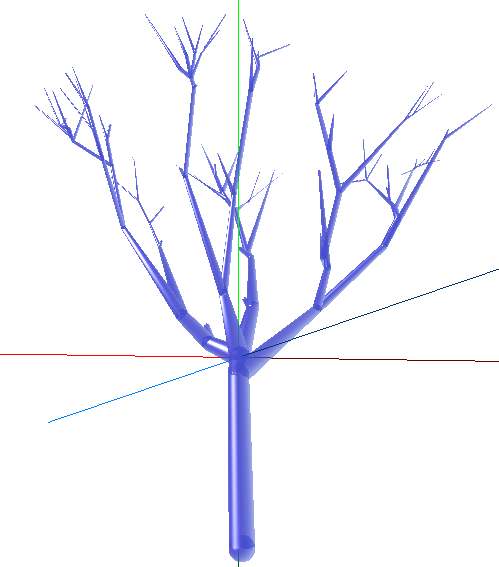
\includegraphics[width=0.4\linewidth]{uc6_2.png}}\hfill
	\caption{用例图示:简化模型}
	\label{fig:uc6}
\end{figure}

\begin{table}[H]
	\centering
\begin{tabular}{|l|p{8cm}|}
	\hline
	用例名称: & 简化模型\\
	\hline
	用例标志号: & 6\\
	\hline
	参与者: & 用户\\
	\hline
	简要说明: & 用户可以通过选择某棵子树,对其进行如第\ref{cha:branchcombine}章中的合并操作,以简化模型。具体效果见图\ref{fig:uc6}\\
	\hline
	前置条件: & 树木的显示模式为骨架模型\\
	\hline
	基本事件流: & 1. 用户按下's'键\\
	 & 2. 对当前节点及其表示的子树进行基于合并的简化\\
	 & 3. 用例终止\\
	\hline
	后置条件: & 无\\
	\hline
\end{tabular}
\end{table}

\clearpage
\subsection{泛洪算法演示}
\begin{figure}[H]
	\centering
	\subfloat[输入:从点云中得到的体素模型]{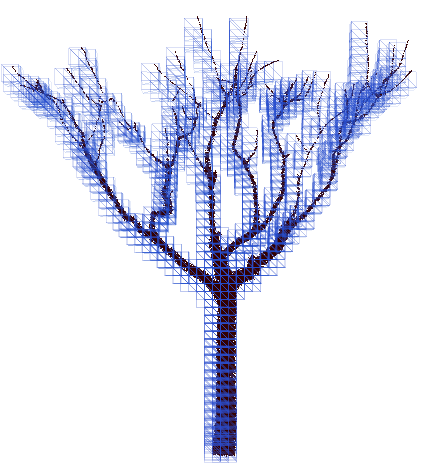
\includegraphics[width=0.26\linewidth]{uc7_1.png}}\hfill
	\subfloat[第1次迭代]{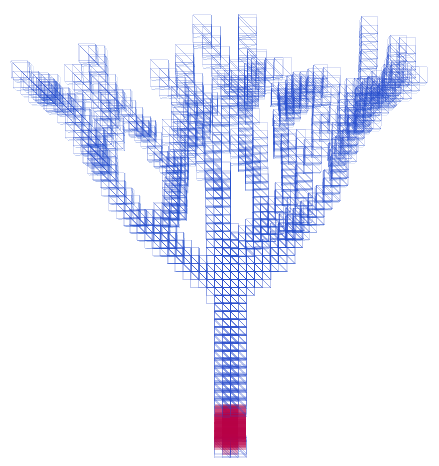
\includegraphics[width=0.26\linewidth]{uc7_2.png}}\hfill
	\subfloat[第4次迭代]{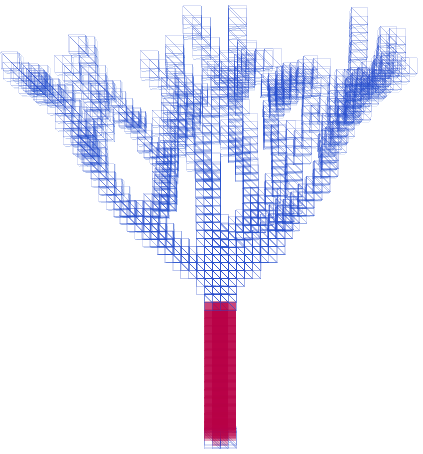
\includegraphics[width=0.26\linewidth]{uc7_3.png}}\hfill
	\subfloat[第7次迭代]{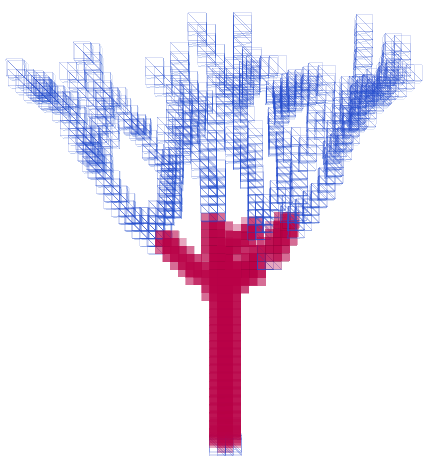
\includegraphics[width=0.26\linewidth]{uc7_4.png}}\hfill
	\subfloat[第10次迭代]{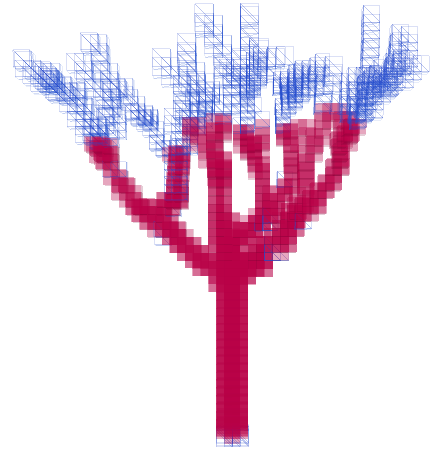
\includegraphics[width=0.26\linewidth]{uc7_5.png}}\hfill
	\subfloat[泛洪算法完成]{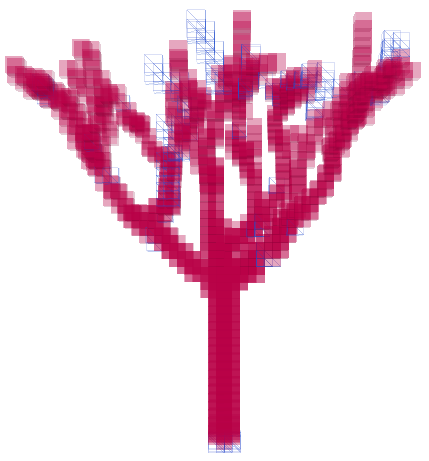
\includegraphics[width=0.26\linewidth]{uc7_6.png}}
	\caption{用例图示:泛洪算法演示}
	\label{fig:uc7}
\end{figure}

\begin{table}[H]
	\centering
\begin{tabular}{|l|p{8cm}|}
	\hline
	用例名称: & 泛洪算法演示\\
	\hline
	用例标志号: & 7\\
	\hline
	参与者: & 用户\\
	\hline
	简要说明: & 用户可以根据输入的点云,进行泛洪算法的可视化单步观察。具体效果见图\ref{fig:uc7}\\
	\hline
	前置条件: & 树木的点云数据已经被加载进入程序,并且打开了体素模型模式\\
	\hline
	基本事件流: & 1. 用户按下'e'键\\
	 & 2. 对当前节点进行泛洪并找到其字节点\\
	 & 3. 选中其子节点,并重复1和2中的步骤\\
	 & 4. 当达到叶子节点时,用例结束\\
	\hline
	后置条件: & 无\\
	\hline
\end{tabular}
\end{table}

\clearpage
\section{利用用户交互提升算法完整性}
根据用户交互平台提供的一系列功能,可以对本文提出的骨架抽取算法进行进一步的完善。由于依靠自动化
骨架抽取算法不可能100\%的恢复出树木的骨架信息,它可能带有一定的骨架缺失,因此有必要依靠少量的人工
交互与指引,进一步完善算法中的缺失部分,从而得到一个完整的骨架模型。这里的人工指引并不是指的逐
个节点的手工编辑,而是对某些缺失的骨架给出一个方向的指引,使得其在缺失方向上重新进行泛洪,而自动化
地补全缺失的信息。这种方式比起手工对缺失的骨架进行建模效率高出许多,因为用户只要给出一个缺失的方向
即可。

图\ref{fig:intalg}展示了通过用户交互的方法指引泛洪算法的进一步完善的过程。
如图\ref{fig:intalg}(a),该树木模型已经经过了本文前文所介绍的骨架抽取步骤。然而与点云模型相对比,
发现当前节点处仍有部分的枝干丢失。经过分析,该枝干丢失可能的原因主要是骨架抽取算法的分支判定条件
并没有将当前分支判定进去。一种可行的办法是调整分支条件的参数,但是这对于用户来说并不是一种很好
的解决办法,因为在实际应用中,要用户去了解一个算法内部的参数是不大可能的。因此本文提出了基于用户
交互与指引的方法,用户只需要从缺失枝干的父枝干出发,引出一个子节点,而泛洪算法将由该子节点开始
继续探索该缺失部分。图\ref{fig:intalg}(b)给出了一个用户指引生成的节点,因此泛洪算法将继续从该
子节点开始,恢复该缺失枝条的骨架。最终的恢复结果如图\ref{fig:intalg}(c)所示。其中橙色球体代表当前
节点,红色区域代表点云,褐色区域代表已抽取骨架,蓝色区域代表通过用户交互恢复出来的枝条。

\begin{figure}[H]
	\centering
	\subfloat[缺失的枝条]{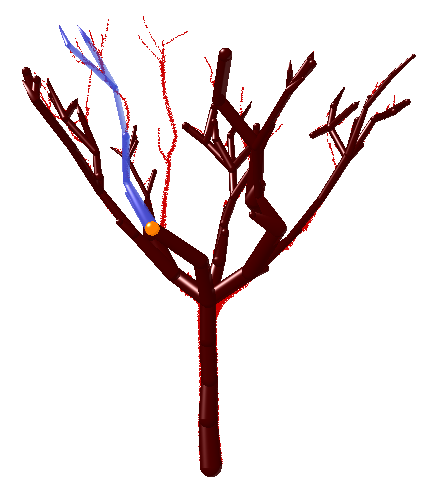
\includegraphics[width=0.3\linewidth]{before.png}}\hfill
	\subfloat[新插入节点作为算法指引]{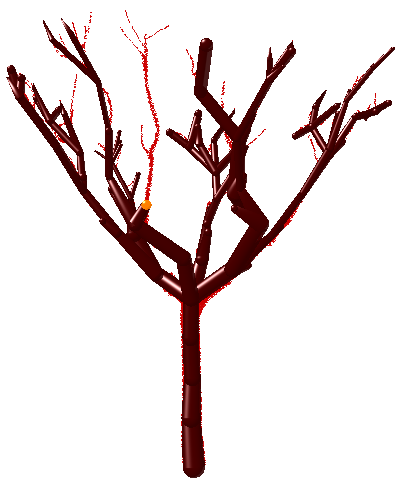
\includegraphics[width=0.3\linewidth]{direction.png}}\hfill
	\subfloat[恢复的枝条]{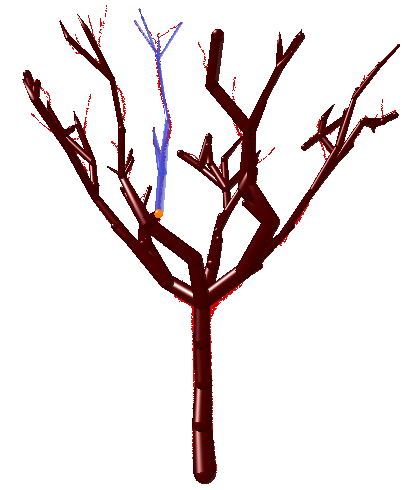
\includegraphics[width=0.3\linewidth]{after.png}}
	\caption{基于用户交互提升算法完整性}
	\label{fig:intalg}
\end{figure}

可见,基于用户交互对算法进行快捷而方便的指引,相较于让用户逐个节点去进行完善,这种方法对于缺失枝干
的恢复具有重要意义。首先,该方法只用引出一个节点作为新的种子点,泛洪算法就可以递归性地恢复整个枝干,
这比起让用户去逐个节点的编辑,大大的节省了建模的时间;同时,由于运用本文介绍的骨架抽取算法所抽取出
的骨架已经大部分的还原了原始骨架,因此需要的用户交互只是及其少量的,这就保证了建模还是由自动化的方法
主导的,有着很好的便捷性;最后,若用户对于最终恢复的模型还有局部需要微调,则可以配合前面的模型编辑
功能进行编辑,这种编辑是建立在已经成型的树木骨架的基础上的,因此比起从头开始建模,也是更加方便和
快捷的方式。

\section{本章小节}
本章给出了一个基于用户交互的模型改善平台,它可以解决自动化算法所带来的一些主观性和二义性问题,通过
最终用户或应用来对自动化生成的模型进行改善,可以使本文给出的基于图像的树木轻量化算法普及到更多的应用
和需求。该平台集成了加载树木点云文件、显示骨架模型、显示点云模型、显示体素模型、节点编辑、简化模型、
以及算法演示的功能,能够很方便和快捷地对自动化生成的模型进行观察和加工。本章还给出了各个功能具体的
用例图和表格加以说明。
